% latex table generated in R 3.2.0 by xtable 1.7-4 package
% Sun Jun 21 15:26:40 2015
\begin{longtable}{lL{1.8cm}C{2cm}ccc}
\caption[Number of taxa with available cladistic data for mammalian orders]{Number of taxa with available cladistic data for mammalian orders at three taxonomic levels. The left vertical bar represents ``low'' coverage (\textless 25\%); the right vertical bar represents ``high'' coverage (\textgreater 75\%). A negative Net Relatedness Index (NRI) and Nearest Taxon Index (NTI) shows more phylogeneticaly dispersed taxa than expected by chance; a positive value shows more phylogeneticaly clustered taxa than expected by chance. Significant NRI or NTI values are highlighted in bold. *p \textless 0.05; **p \textless 0.01; ***p \textless 0.001.} \\ 
  \hline
\textbf{Order} & \textbf{Taxonomic level} & \textbf{Proportion of taxa} & \textbf{Coverage} & \textbf{NRI} & \textbf{NTI} \\ 
  \hline
Afrosoricida & family & 2/2 & 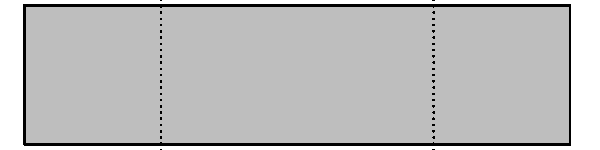
\includegraphics[width=0.20\linewidth, height=0.05\linewidth]{Missing_mammals/Table_figures/bar1.pdf} &   &   \\ 
  Afrosoricida & genus & 17/17 & 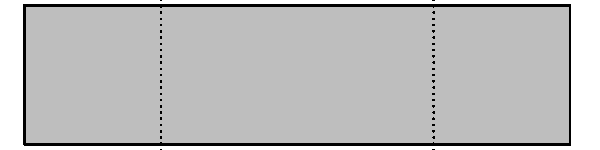
\includegraphics[width=0.20\linewidth, height=0.05\linewidth]{Missing_mammals/Table_figures/bar2.pdf} &   &   \\ 
  \textbf{Afrosoricida} & \textbf{species} & \textbf{23/42} & 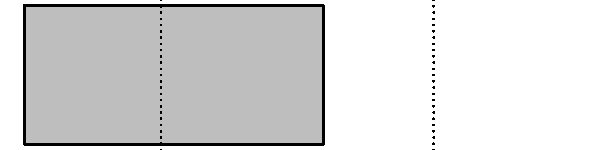
\includegraphics[width=0.20\linewidth, height=0.05\linewidth]{Missing_mammals/Table_figures/bar3.pdf} & \textbf{1.89*} & 1.19 \\ 
  Carnivora & family & 11/15 & 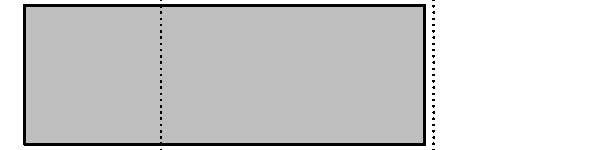
\includegraphics[width=0.20\linewidth, height=0.05\linewidth]{Missing_mammals/Table_figures/bar4.pdf} & 0.43 & 1.68 \\ 
  \textbf{Carnivora} & \textbf{genus} & \textbf{30/125} & 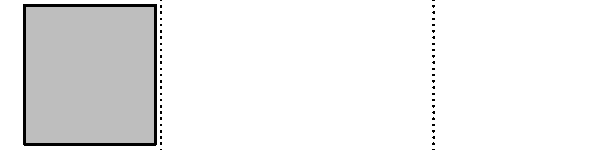
\includegraphics[width=0.20\linewidth, height=0.05\linewidth]{Missing_mammals/Table_figures/bar5.pdf} & \textbf{4.14**} & \textbf{1.81*} \\ 
  \textbf{Carnivora} & \textbf{species} & \textbf{42/283} & 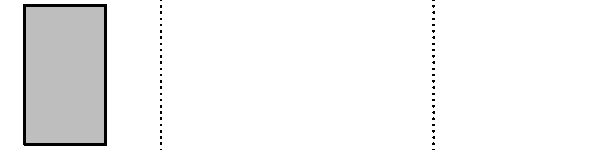
\includegraphics[width=0.20\linewidth, height=0.05\linewidth]{Missing_mammals/Table_figures/bar6.pdf} & \textbf{18.64**} & \textbf{3.02**} \\ 
  Cetartiodactyla & family & 21/21 & 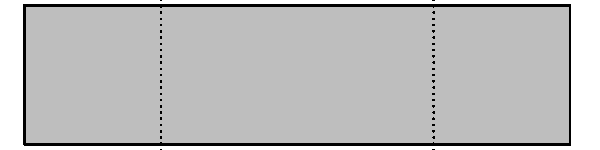
\includegraphics[width=0.20\linewidth, height=0.05\linewidth]{Missing_mammals/Table_figures/bar7.pdf} &   &   \\ 
  \textbf{Cetartiodactyla} & \textbf{genus} & \textbf{77/128} & 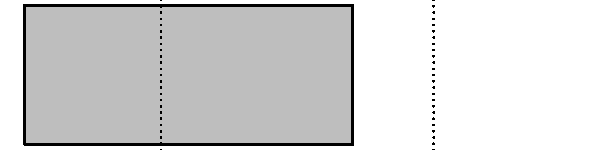
\includegraphics[width=0.20\linewidth, height=0.05\linewidth]{Missing_mammals/Table_figures/bar8.pdf} & 0.87 & \textbf{1.77*} \\ 
  \textbf{Cetartiodactyla} & \textbf{species} & \textbf{129/310} & 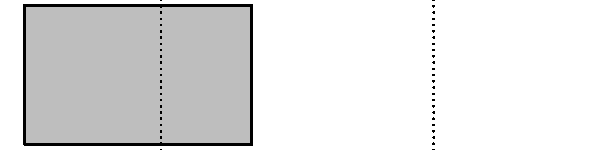
\includegraphics[width=0.20\linewidth, height=0.05\linewidth]{Missing_mammals/Table_figures/bar9.pdf} & \textbf{2.72*} & 0.04 \\ 
  Chiroptera & family & 13/18 & 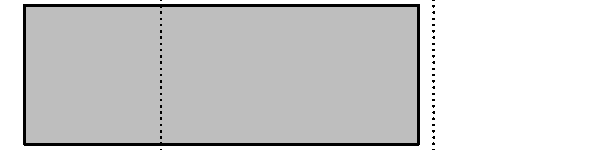
\includegraphics[width=0.20\linewidth, height=0.05\linewidth]{Missing_mammals/Table_figures/bar10.pdf} & 0.55 & 0.63 \\ 
  \textbf{Chiroptera} & \textbf{genus} & \textbf{85/202} & 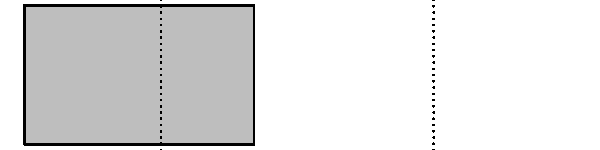
\includegraphics[width=0.20\linewidth, height=0.05\linewidth]{Missing_mammals/Table_figures/bar11.pdf} & \textbf{16.91**} & \textbf{2.85**} \\ 
  \textbf{Chiroptera} & \textbf{species} & \textbf{165/1053} & 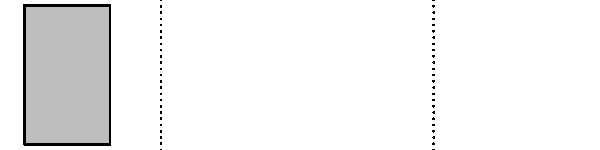
\includegraphics[width=0.20\linewidth, height=0.05\linewidth]{Missing_mammals/Table_figures/bar12.pdf} & \textbf{14.55**} & \textbf{3.44**} \\ 
  Cingulata & family & 1/1 & 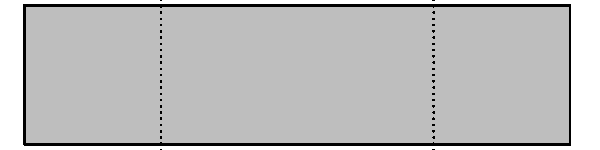
\includegraphics[width=0.20\linewidth, height=0.05\linewidth]{Missing_mammals/Table_figures/bar13.pdf} &   &   \\ 
  Cingulata & genus & 8/9 & 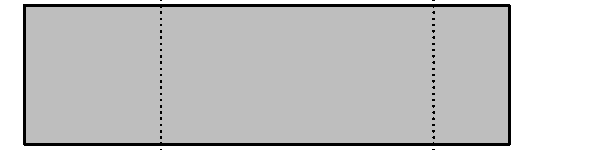
\includegraphics[width=0.20\linewidth, height=0.05\linewidth]{Missing_mammals/Table_figures/bar14.pdf} & 1.49 & -1.63 \\ 
  Cingulata & species & 6/29 & 
\includegraphics[width=0.20\linewidth, height=0.05\linewidth]{Missing_mammals/Table_figures/bar15.pdf} & 1.43 & 0.36 \\ 
  Dasyuromorphia & family & 2/2 & 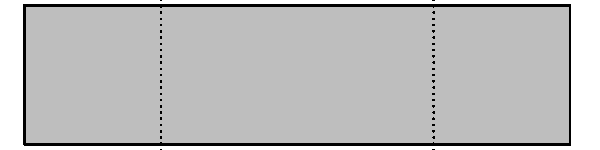
\includegraphics[width=0.20\linewidth, height=0.05\linewidth]{Missing_mammals/Table_figures/bar16.pdf} &   &   \\ 
  Dasyuromorphia & genus & 7/22 & 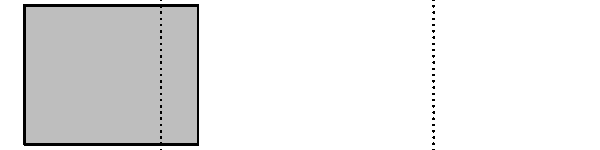
\includegraphics[width=0.20\linewidth, height=0.05\linewidth]{Missing_mammals/Table_figures/bar17.pdf} & -1 & -1.45 \\ 
  Dasyuromorphia & species & 8/64 & 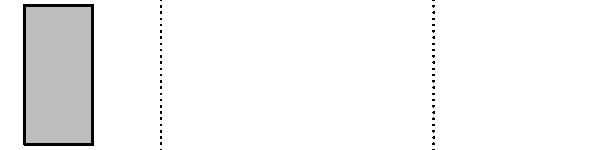
\includegraphics[width=0.20\linewidth, height=0.05\linewidth]{Missing_mammals/Table_figures/bar18.pdf} & -1.15 & -0.62 \\ 
  Dermoptera & family & 1/1 & 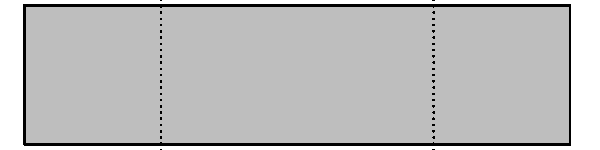
\includegraphics[width=0.20\linewidth, height=0.05\linewidth]{Missing_mammals/Table_figures/bar19.pdf} &   &   \\ 
  Dermoptera & genus & 1/2 & 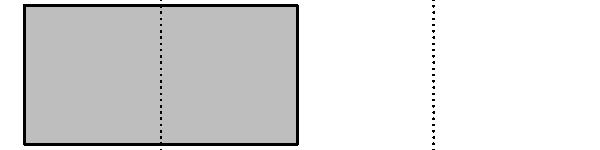
\includegraphics[width=0.20\linewidth, height=0.05\linewidth]{Missing_mammals/Table_figures/bar20.pdf} &   &   \\ 
  Dermoptera & species & 1/2 & 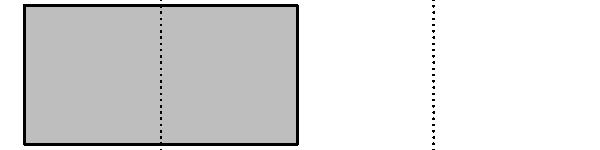
\includegraphics[width=0.20\linewidth, height=0.05\linewidth]{Missing_mammals/Table_figures/bar21.pdf} &   &   \\ 
  Didelphimorphia & family & 1/1 & 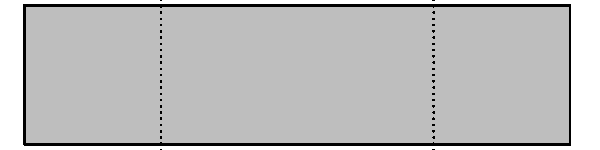
\includegraphics[width=0.20\linewidth, height=0.05\linewidth]{Missing_mammals/Table_figures/bar22.pdf} &   &   \\ 
  Didelphimorphia & genus & 16/16 & 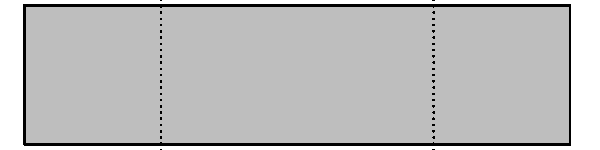
\includegraphics[width=0.20\linewidth, height=0.05\linewidth]{Missing_mammals/Table_figures/bar23.pdf} &   &   \\ 
  Didelphimorphia & species & 40/84 & 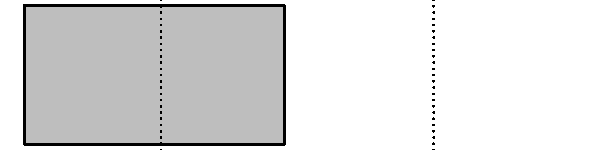
\includegraphics[width=0.20\linewidth, height=0.05\linewidth]{Missing_mammals/Table_figures/bar24.pdf} & -0.94 & 0.36 \\ 
  Diprotodontia & family & 9/11 & 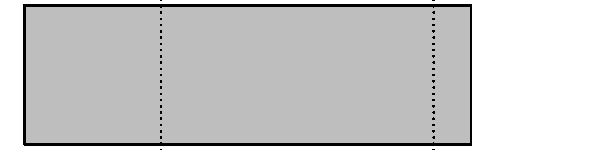
\includegraphics[width=0.20\linewidth, height=0.05\linewidth]{Missing_mammals/Table_figures/bar25.pdf} & -0.8 & 0.56 \\ 
  Diprotodontia & genus & 20/38 & 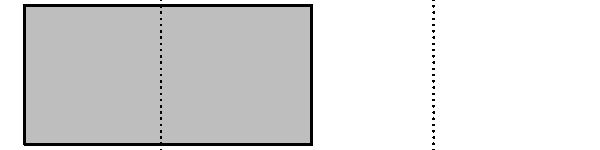
\includegraphics[width=0.20\linewidth, height=0.05\linewidth]{Missing_mammals/Table_figures/bar26.pdf} & -1.36 & -0.73 \\ 
  Diprotodontia & species & 16/126 & 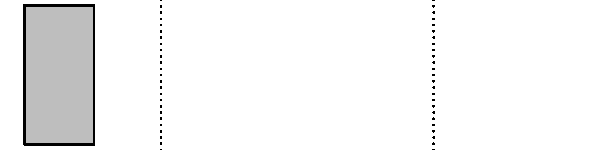
\includegraphics[width=0.20\linewidth, height=0.05\linewidth]{Missing_mammals/Table_figures/bar27.pdf} & -2.29 & -1.55 \\ 
  Erinaceomorpha & family & 1/1 & 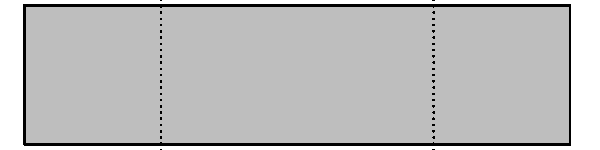
\includegraphics[width=0.20\linewidth, height=0.05\linewidth]{Missing_mammals/Table_figures/bar28.pdf} &   &   \\ 
  Erinaceomorpha & genus & 10/10 & 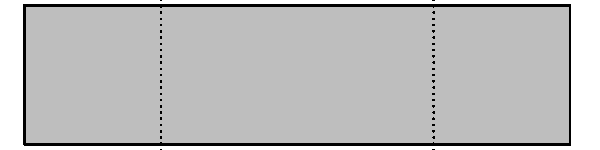
\includegraphics[width=0.20\linewidth, height=0.05\linewidth]{Missing_mammals/Table_figures/bar29.pdf} &   &   \\ 
  Erinaceomorpha & species & 21/22 & 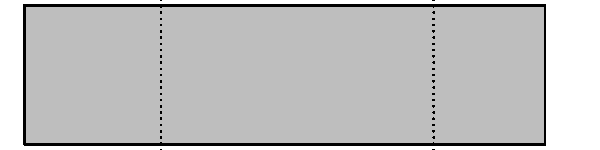
\includegraphics[width=0.20\linewidth, height=0.05\linewidth]{Missing_mammals/Table_figures/bar30.pdf} & -1.1 & -0.3 \\ 
  Hyracoidea & family & 1/1 & 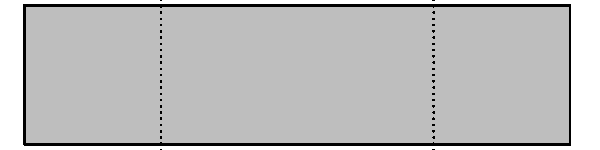
\includegraphics[width=0.20\linewidth, height=0.05\linewidth]{Missing_mammals/Table_figures/bar31.pdf} &   &   \\ 
  Hyracoidea & genus & 1/3 & 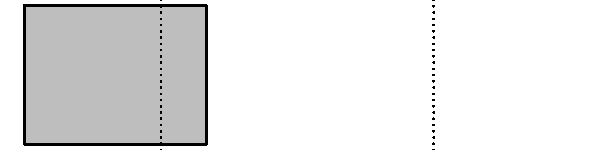
\includegraphics[width=0.20\linewidth, height=0.05\linewidth]{Missing_mammals/Table_figures/bar32.pdf} &   &   \\ 
  Hyracoidea & species & 1/4 & 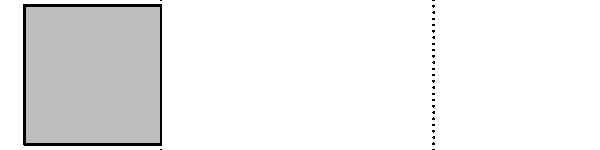
\includegraphics[width=0.20\linewidth, height=0.05\linewidth]{Missing_mammals/Table_figures/bar33.pdf} &   &   \\ 
  Lagomorpha & family & 1/2 & 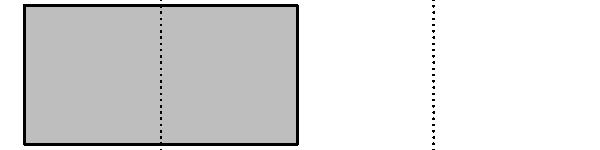
\includegraphics[width=0.20\linewidth, height=0.05\linewidth]{Missing_mammals/Table_figures/bar34.pdf} &   &   \\ 
  Lagomorpha & genus & 1/12 & 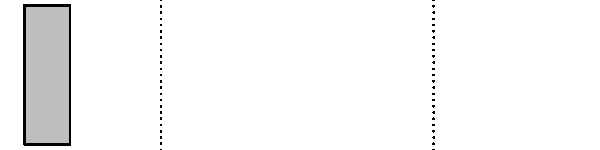
\includegraphics[width=0.20\linewidth, height=0.05\linewidth]{Missing_mammals/Table_figures/bar35.pdf} &   &   \\ 
  Lagomorpha & species & 1/86 & 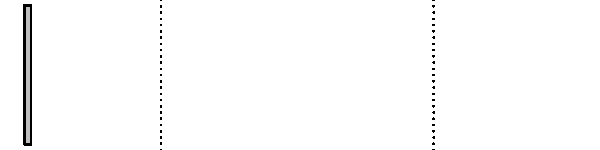
\includegraphics[width=0.20\linewidth, height=0.05\linewidth]{Missing_mammals/Table_figures/bar36.pdf} &   &   \\ 
  Macroscelidea & family & 1/1 & 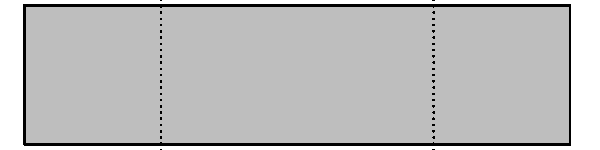
\includegraphics[width=0.20\linewidth, height=0.05\linewidth]{Missing_mammals/Table_figures/bar37.pdf} &   &   \\ 
  Macroscelidea & genus & 4/4 & 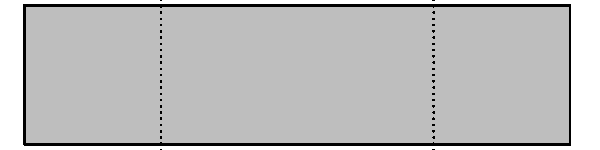
\includegraphics[width=0.20\linewidth, height=0.05\linewidth]{Missing_mammals/Table_figures/bar38.pdf} &   &   \\ 
  Macroscelidea & species & 5/15 & 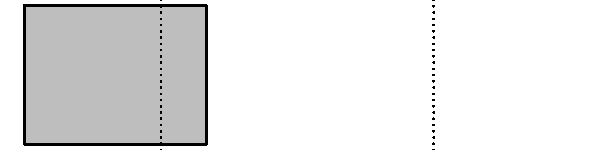
\includegraphics[width=0.20\linewidth, height=0.05\linewidth]{Missing_mammals/Table_figures/bar39.pdf} & -0.98 & -1.38 \\ 
  Microbiotheria & family & 1/1 & 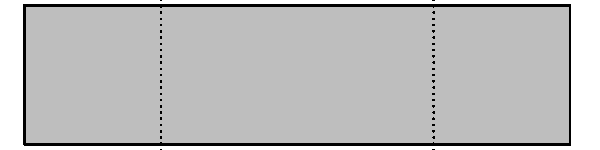
\includegraphics[width=0.20\linewidth, height=0.05\linewidth]{Missing_mammals/Table_figures/bar40.pdf} &   &   \\ 
  Microbiotheria & genus & 1/1 & 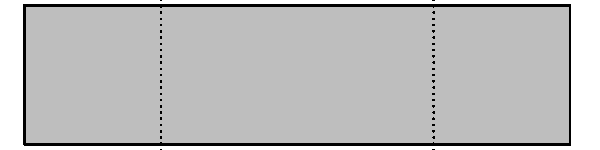
\includegraphics[width=0.20\linewidth, height=0.05\linewidth]{Missing_mammals/Table_figures/bar41.pdf} &   &   \\ 
  Microbiotheria & species & 1/1 & 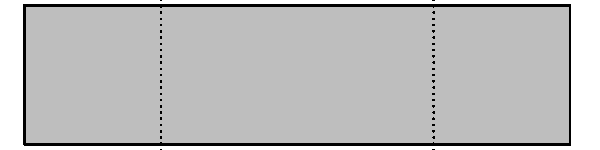
\includegraphics[width=0.20\linewidth, height=0.05\linewidth]{Missing_mammals/Table_figures/bar42.pdf} &   &   \\ 
  Monotremata & family & 2/2 & 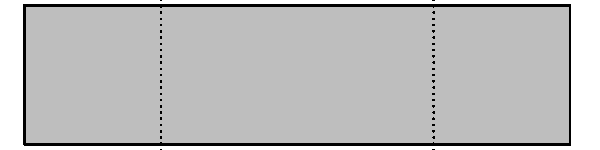
\includegraphics[width=0.20\linewidth, height=0.05\linewidth]{Missing_mammals/Table_figures/bar43.pdf} &   &   \\ 
  Monotremata & genus & 2/3 & 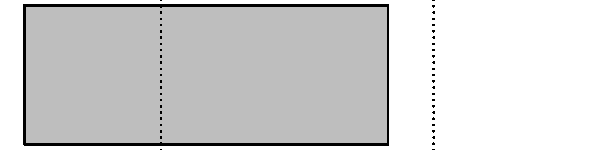
\includegraphics[width=0.20\linewidth, height=0.05\linewidth]{Missing_mammals/Table_figures/bar44.pdf} & -0.71 & -0.71 \\ 
  Monotremata & species & 2/4 & 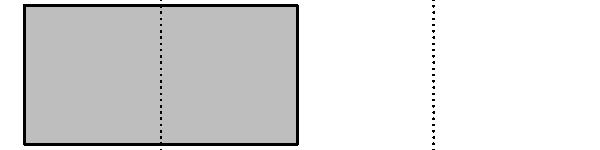
\includegraphics[width=0.20\linewidth, height=0.05\linewidth]{Missing_mammals/Table_figures/bar45.pdf} & -1.01 & -1.03 \\ 
  Notoryctemorphia & family & 1/1 & 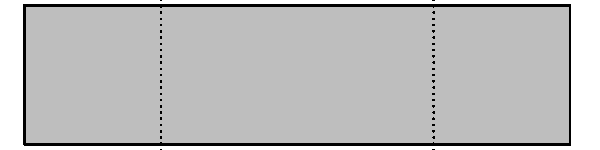
\includegraphics[width=0.20\linewidth, height=0.05\linewidth]{Missing_mammals/Table_figures/bar46.pdf} &   &   \\ 
  Notoryctemorphia & genus & 1/1 & 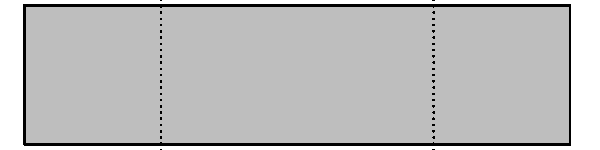
\includegraphics[width=0.20\linewidth, height=0.05\linewidth]{Missing_mammals/Table_figures/bar47.pdf} &   &   \\ 
  Notoryctemorphia & species & 0/2 & 
\includegraphics[width=0.20\linewidth, height=0.05\linewidth]{Missing_mammals/Table_figures/bar48.pdf} &   &   \\ 
  Paucituberculata & family & 1/1 & 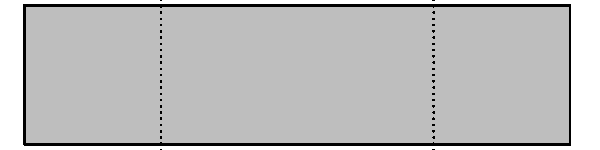
\includegraphics[width=0.20\linewidth, height=0.05\linewidth]{Missing_mammals/Table_figures/bar49.pdf} &   &   \\ 
  Paucituberculata & genus & 2/3 & 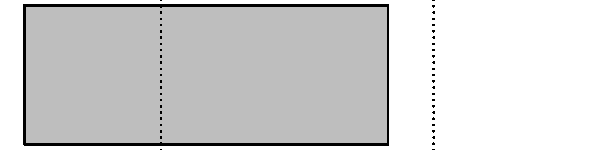
\includegraphics[width=0.20\linewidth, height=0.05\linewidth]{Missing_mammals/Table_figures/bar50.pdf} & 0 & 0 \\ 
  Paucituberculata & species & 2/5 & \includegraphics[width=0.20\linewidth, height=0.05\linewidth]{Missing_mammals/Table_figures/bar51.pdf} & -0.64 & -0.65 \\ 
  Peramelemorphia & family & 2/2 & \includegraphics[width=0.20\linewidth, height=0.05\linewidth]{Missing_mammals/Table_figures/bar52.pdf} &   &   \\ 
  Peramelemorphia & genus & 7/7 & \includegraphics[width=0.20\linewidth, height=0.05\linewidth]{Missing_mammals/Table_figures/bar53.pdf} &   &   \\ 
  Peramelemorphia & species & 16/18 & \includegraphics[width=0.20\linewidth, height=0.05\linewidth]{Missing_mammals/Table_figures/bar54.pdf} & -0.09 & 1 \\ 
  Perissodactyla & family & 3/3 & \includegraphics[width=0.20\linewidth, height=0.05\linewidth]{Missing_mammals/Table_figures/bar55.pdf} &   &   \\ 
  Perissodactyla & genus & 6/6 & \includegraphics[width=0.20\linewidth, height=0.05\linewidth]{Missing_mammals/Table_figures/bar56.pdf} &   &   \\ 
  Perissodactyla & species & 7/16 & \includegraphics[width=0.20\linewidth, height=0.05\linewidth]{Missing_mammals/Table_figures/bar57.pdf} & 0.62 & -2.5 \\ 
  Pholidota & family & 1/1 & \includegraphics[width=0.20\linewidth, height=0.05\linewidth]{Missing_mammals/Table_figures/bar58.pdf} &   &   \\ 
  Pholidota & genus & 1/1 & \includegraphics[width=0.20\linewidth, height=0.05\linewidth]{Missing_mammals/Table_figures/bar59.pdf} &   &   \\ 
  \textbf{Pholidota} & \textbf{species} & \textbf{3/8} & \includegraphics[width=0.20\linewidth, height=0.05\linewidth]{Missing_mammals/Table_figures/bar60.pdf} & \textbf{2.64*} & \textbf{2.23*} \\ 
  Pilosa & family & 3/5 & \includegraphics[width=0.20\linewidth, height=0.05\linewidth]{Missing_mammals/Table_figures/bar61.pdf} & 0.94 & 0.93 \\ 
  Pilosa & genus & 3/5 & \includegraphics[width=0.20\linewidth, height=0.05\linewidth]{Missing_mammals/Table_figures/bar62.pdf} & -0.36 & -0.31 \\ 
  Pilosa & species & 3/29 & \includegraphics[width=0.20\linewidth, height=0.05\linewidth]{Missing_mammals/Table_figures/bar63.pdf} & 0.33 & 0.79 \\ 
  Primates & family & 15/15 & \includegraphics[width=0.20\linewidth, height=0.05\linewidth]{Missing_mammals/Table_figures/bar64.pdf} &   &   \\ 
  Primates & genus & 48/68 & \includegraphics[width=0.20\linewidth, height=0.05\linewidth]{Missing_mammals/Table_figures/bar65.pdf} & -0.41 & -1.4 \\ 
  Primates & species & 56/351 & \includegraphics[width=0.20\linewidth, height=0.05\linewidth]{Missing_mammals/Table_figures/bar66.pdf} & -1.6 & -2.04 \\ 
  Proboscidea & family & 1/1 & \includegraphics[width=0.20\linewidth, height=0.05\linewidth]{Missing_mammals/Table_figures/bar67.pdf} &   &   \\ 
  Proboscidea & genus & 1/2 & \includegraphics[width=0.20\linewidth, height=0.05\linewidth]{Missing_mammals/Table_figures/bar68.pdf} &   &   \\ 
  Proboscidea & species & 1/3 & \includegraphics[width=0.20\linewidth, height=0.05\linewidth]{Missing_mammals/Table_figures/bar69.pdf} &   &   \\ 
  Rodentia & family & 11/32 & \includegraphics[width=0.20\linewidth, height=0.05\linewidth]{Missing_mammals/Table_figures/bar70.pdf} & -0.46 & -1.91 \\ 
  Rodentia & genus & 21/450 & \includegraphics[width=0.20\linewidth, height=0.05\linewidth]{Missing_mammals/Table_figures/bar71.pdf} & -2.11 & 0.3 \\ 
  Rodentia & species & 15/2094 & \includegraphics[width=0.20\linewidth, height=0.05\linewidth]{Missing_mammals/Table_figures/bar72.pdf} & -1.65 & -2.55 \\ 
  Scandentia & family & 2/2 & \includegraphics[width=0.20\linewidth, height=0.05\linewidth]{Missing_mammals/Table_figures/bar73.pdf} &   &   \\ 
  Scandentia & genus & 2/5 & \includegraphics[width=0.20\linewidth, height=0.05\linewidth]{Missing_mammals/Table_figures/bar74.pdf} & -0.77 & -0.76 \\ 
  Scandentia & species & 2/20 & \includegraphics[width=0.20\linewidth, height=0.05\linewidth]{Missing_mammals/Table_figures/bar75.pdf} & -1.79 & -1.99 \\ 
  Sirenia & family & 2/2 & \includegraphics[width=0.20\linewidth, height=0.05\linewidth]{Missing_mammals/Table_figures/bar76.pdf} &   &   \\ 
  Sirenia & genus & 2/2 & \includegraphics[width=0.20\linewidth, height=0.05\linewidth]{Missing_mammals/Table_figures/bar77.pdf} &   &   \\ 
  Sirenia & species & 4/4 & \includegraphics[width=0.20\linewidth, height=0.05\linewidth]{Missing_mammals/Table_figures/bar78.pdf} &   &   \\ 
  Soricomorpha & family & 3/4 & \includegraphics[width=0.20\linewidth, height=0.05\linewidth]{Missing_mammals/Table_figures/bar79.pdf} & -0.93 & -0.92 \\ 
  \textbf{Soricomorpha} & \textbf{genus} & \textbf{19/43} & \includegraphics[width=0.20\linewidth, height=0.05\linewidth]{Missing_mammals/Table_figures/bar80.pdf} & \textbf{6.98**} & \textbf{2.49*} \\ 
  \textbf{Soricomorpha} & \textbf{species} & \textbf{19/392} & \includegraphics[width=0.20\linewidth, height=0.05\linewidth]{Missing_mammals/Table_figures/bar81.pdf} & \textbf{13.19**} & \textbf{3.89**} \\ 
  Tubulidentata & family & 1/1 & \includegraphics[width=0.20\linewidth, height=0.05\linewidth]{Missing_mammals/Table_figures/bar82.pdf} &   &   \\ 
  Tubulidentata & genus & 1/1 & \includegraphics[width=0.20\linewidth, height=0.05\linewidth]{Missing_mammals/Table_figures/bar83.pdf} &   &   \\ 
  Tubulidentata & species & 1/1 & \includegraphics[width=0.20\linewidth, height=0.05\linewidth]{Missing_mammals/Table_figures/bar84.pdf} &   &   \\ 
   \hline
\hline
\label{Table_results}
\end{longtable}
